
After completing this chapter, you should be able to:

\begin{enumerate}
 \item Explain Hooke's Law in regards to mass-spring systems. Construct and solve differential equations that model spring motion, with or without the presence of a damper.  
 \item Speak using the vocabulary and language of higher order ODEs, such as homogeneous, linear, coefficients, superposition principle, basis of solutions, Wronskian, etc. 
 \item Use Laplace transforms and $s$-shifting to solve homogeneous IVPs.
 \item Use eigenvalues and eigenvectors to solve homogeneous ODE's. Show how to solve IVPs with $\vec y = QDQ^{-1}\vec y(0)$. 
 \item Explain how to immediately jump from the characteristic polynomial to the solution of a homogeneous ODE.
\end{enumerate}






%Should I split up the problems into their own files? No.  I would rather name each problem and then sort them.  That sounds much better. 


\renewcommand{\ideaA}{Building Mathematical Models}
\renewcommand{\ideaB}{Solving Higher Order ODEs}
\renewcommand{\ideaC}{Solving Systems of ODEs with Eigenvalues and Eigenvectors}
\renewcommand{\ideaD}{The theory of homogeneous differential equations}



\mysubsection{\ideaA}

In this chapter, we're going to learn how to solve a huge collection of higher order differential equations.  Before diving into the details, let's make sure we know WHY we would even want to do so. If I knew you all had the same background, we could dive into lots of examples directly related to your field (you'll do that in future classes in your major).  Since we have a diverse background in our class, we'll stick mostly to models that connect velocity, position, and acceleration.  Before the next chapter ends, we'll add to this some information about electrical circuits.


For our first model, let's look at how we can obtain the position of an object in projectile motion from knowledge about the acceleration and velocity.  You've solve this problem before, but the solution required neglecting air resistance. 
\begin{example}
In multivariate calculus, we encountered the differential equation $y''=-g$. In this differential equation, the only force $F_T=my''$ acting on an object in projectile motion is the force of gravity $F_G=-mg$. Equating these two gives us the ODE $my''=-mg$, or just $y''=-g$.  If we have initial position $y(0)=y_0$ and initial speed $y'(0)=v_0$, then the solution is $y=-\frac{1}{2}gt^2+v_0t+y_0$. We found that solution by integrating twice. 
\end{example}
We don't have to neglect air resistance anymore.  We could talk about sky diving (risky), dropping bombs (deadly), throwing math books off a roof (illegal), putting a satellite into geosynchronous orbit (useful), or dropping a pebble from the top of a waterfall (head to Yellowstone and try it - sounds like we need a field trip). The next problem asks you to revisit the example above, but now add in air resistance.
\begin{problem}\label{pebble from falls}
 Joe hikes up to the top of Lower Falls in Yellowstone.  His hope is to gauge the height $h$ of the waterfall.  He plans to drop a pebble from the top, and time how long it takes for the pebble to hit the ground. He'll need a model that predicts the height of the pebble at any time $t$.

 For this to work, Joe has to make some assumptions.  His assumptions might be way off, but that's how science works. We start with assumptions and then turn those assumptions into differential equations. Here's what Joe assumes:
\begin{itemize}
 \item He assumes Newton's second law of motion, namely that $F=ma$ (the total force is the mass times the acceleration).
 \item He assumes that the total force is comprised of two parts.  
 \item The first force $F_G$ comes from a constant acceleration due to gravity. He assumes that gravity is constant $a=-g$. The negative sign comes because the acceleration causes a decrease in height.
 \item The second part comes from air resistance. He assumes that the faster the pebble goes, the greater this force will be. If the pebble's speed were to double, then this force should double.  So he assumes that the force due to air resistance $F_R$ is proportional to the pebble's velocity.
\end{itemize}
Let $y(t)$ represent the height, above ground, of the pebble after $t$ seconds. Use Joe's assumptions to answer the following:
\begin{enumerate}
 \item Rewrite Newton's second law of motion in terms of $y$, $y'$, and/or $y''$. 
 \item What is the constant force $F_G$ due to gravity?
 \item Rewrite Joe's assumption about air resistance in terms of $y$, $y'$ and/or $y''$. 
 \item The total force $F$ is the sum of the two forces, i.e. we can write $F = F_G+F_R$. Use this fact, together with your answers from the previous parts, to obtain a second order ODE.  You don't have to solve the ODE, rather you just need to obtain it.
 \item If we let $y'=v$ so that $v'=y''$, then show how to rewrite your ODE above in the matrix form 
$$\bvec{y'\\v'} = \bvec{0&1\\0&-k/m}\bvec{y\\v}+\bvec{0\\-g}.$$
\end{enumerate}
If you need any hints, try searching the web for ``modeling motion if we assume that air resistance is proportional to speed.''
\end{problem}

Congrats.  You've just set up your first second order ODE. 
Let's now look at another position/velocity/acceleration model, but this time related to springs. 
We'll start by considering the following scenario. We attach an object with mass $m$ to a spring.  
\marginpar{In the next chapter, we'll hang the spring from a ceiling. In this case, we'll have an additional force $F_g=-mg$ acting on the spring.}
We place the spring horizontally, and put the mass on a frictionless track. We let go of the object, and allow it to come to rest. We'll use the function $x(t)$ to keep track of the position of the spring at any time $t$, with $x=0$ corresponding to equilibrium (the mass is at rest). Robert Hooke (1635 -- 1703) developed the following law, called Hooke's law:
\begin{quote}
 The force needed to extend (or compress) a spring a distance $x$ is proportional to the distance $x$. Note that the force acts opposite the displacement.
\end{quote}
\begin{problem}
 Read the preceding paragraph.  Then answer the following:
\begin{itemize}
 \item Draw a picture of a horizontal track. On the left end of the track, put a wall. Put an object, like a square block, in the center of your track and draw a spring that connects the wall to the block.
 \item Explain why $mx''(t)=-kx(t)$. We generally just write $mx''=-kx$ (the $t$ is assumed).  
 \item If it takes $8 \text{ N} = 8$kg m/s$^2$ to move the object whose mass is 4 kg about $.3$ m, what is the spring constant $k$?  How far would a $12$ N force cause the object to move? Does the mass of the object matter?
\end{itemize}
\end{problem}

Hooke's law is not a perfect model for all springs, but it does a good job for most, provided the displacement is not too large.  If the displacements are too large, then the spring may deform, which changes the properties of the spring in all future computations.  If you take your car out onto extremely bumpy roads, and purposefully hit some nasty bumps, you could permanently damage the shocks. In this case, you would want to replace your springs.

Every linear spring has a spring constant $k$. This constant has many names, such as the spring modulus, Young's modulus, Young's constant, and more. The next problem shows you how to obtain the spring constant $k$.
\begin{problem}
 You attach a spring to the ceiling. You attach a mass of 10 kg on the end, and the spring elongates 3 cm.  
\begin{enumerate}
 \item You now attach a mass of 20 kg. How long will the spring elongate? 
 \item What is the spring constant $k$? Give the units.
 \item We attach a different spring, and hang the same 10 kg on the end, but this time the spring elongates 2 cm.  Is the spring constant larger or smaller?
 \item If a spring has really large modulus, will it be easy or hard to elongate it?
\end{enumerate}
\end{problem}

We need one more model before we start solving some ODEs.  We'll use the exact same spring model as before. Place a horizontal spring whose modulus is $k$ on a frictionless track. Attach an object whose mass is $m$ to the end of the spring.  
\marginpar{We don't have to place the spring underwater to get the same affect.  We could use a dashpot to resist the motion. One type of dashpot is a cylindrical tube placed around a cylindrical object, so that as the object moves, its sides come in contact with the dashpot, resulting in friction that resists motion. See \href{http://en.wikipedia.org/wiki/Dashpot}{Wikipedia} for more info.}
We now place the entire mass-spring system underwater. When it was exposed to air, we neglected air resistance. Now we'll have to take resistance into account.   
\begin{problem}\label{mass-spring set up problem}
 When we have no resistance, the mass-spring system ODE is $F_T=F_S$, or $mx'' = -kx$.  Assume that the liquid applies a resistive force that is proportional to the velocity of the object.  If the object is resting, the liquid doesn't apply a force.  If you double the speed, then the resistive force doubles.  If you triple the speed, the resistive force triples. 
\begin{enumerate}
 \item Modify the second order ODE $mx''=-kx$ to account for the resistive force of water. 
 \item Then show that we can write this 2nd order ODE as a system of ODEs in the matrix form
$$\bvec{x'\\v'} = \bvec{0&1\\-k/m&-c/m}\bvec{x\\v}.$$

\end{enumerate}

\end{problem}












\mysubsection{\ideaC}


We will need to perform lots of partial fraction decompositions in the next few problems. It would be nice if we had a really easy way to perform them symbolically. Row reduction and Cramer's rule will be our friends. Start by completing the following problem, which is a slight adaptation of a problem from the previous chapter.

\begin{problem}

Consider the partial fraction decomposition 
$$
\frac{8s+7}{(s-2)(s+3)} = \frac{A}{s-2}+\frac{B}{s+3}
$$
which we  can rewrite in the form
$$8s+7 = A(s+3)+B(s-2).$$
\begin{enumerate}
 \item Complete this decomposition (find $A$ and $B$). Use any method you like. 
 \item Now let's solve 
$$
\frac{cs+d}{(s-2)(s+3)} = \frac{A}{s-2}+\frac{B}{s+3}
$$
Rather than thinking of $c$ and $d$ as known constants, let's make them variables in our linear system of equations.  
Our goal is to solve 
$$
cs+d=(A+B)s+(3A-2B)
\quad \text{or}\quad
(A+B-c)s+(3A-2B-d)=0
$$   
which we can rewrite in the matrix form 
\marginpar{Why did I save the last two columns for $c$ and $d$?}%
$$\bvec{
1 & 1 & -1 & 0 \\
3 & -2 & 0 & -1
}\bvec{A\\B\\c\\d}=\bvec{0\\0}.$$
This is a matrix equation of the form $M\vec x=\vec 0$. Find a basis for the kernel of the matrix $M$.
\item 
Change the 2 by 4 matrix above to solve the partial fraction decomposition
$$
\frac{cs+d}{(s-p)(s-q)} = \frac{A}{s-p}+\frac{B}{s-q}.
$$
Find the kernel of this 2 by 4 matrix (use software). Then state $A$ and $B$ in terms of $c$, $d$, $p$, and $q$. 
\item Use Cramer's rule to quickly solve 
$$\bvec{
1 & 1 \\
-q & -p 
}
\bvec{A\\B}
=\bvec{c\\d}$$
and verify that your answer in part 3 is correct.  Under what circumstances would your answer not be valid?
\end{enumerate}
\end{problem}






You'll find that either row reduction with software that can handle symbolic entries (both Sage and Mathematica can do this), or using of Cramer's Rule, will greatly simplify lots of the work we need to do below. You've proven the following theorem.
\begin{theorem}\label{general partial fraction decomposition for a quadratic}
If $p\neq q$, the solution to the partial fraction decomposition
$$
\frac{cs+d}{(s-p)(s-q)} = \frac{A}{s-p}+\frac{B}{s-q}
\quad\text{is}\quad 
A=\frac{-cp-d}{q-p}, \quad B=\frac{cq+d}{q-p}.$$
\end{theorem}
















\begin{problem}
 Consider the system of ODEs
$$
\begin{array}{c}
 x' = 2x+3y\\
 y' = 5x+4y
\end{array}
\quad\Rightarrow\quad
\bvec{x'\\y'} =\bvec{2&3\\5&4}\bvec{x\\y} 
\quad\Rightarrow\quad
\dfrac{d\vec{x}}{dt} =A\vec x. 
$$
\begin{enumerate}
 \item Find the eigenvalues of $A$. Then find a basis for each eigenspace (i.e. find an eigenvector corresponding to each eigenvector). Pick vectors for your bases that do not have fractions in them (rescale if needed).
 \item Recall that the Laplace transforms of each equation are
$$
\begin{array}{c}
 sX-x_0 = 2X+3Y\\
 sY-y_0 = 5X+4Y
\end{array}
\quad\Rightarrow\quad
\begin{array}{c}
 -x_0 = (2-s)X+3Y\\
 -y_0 = 5X+(4-s)Y
\end{array},
$$
where $X$ is the Laplace transform of $x(t)$ and $Y$ is the Laplace transform of $y(t)$. 
Solve for $X$ and $Y$ (Cramer's rule should make this super fast). Do you see any connections between your solution here and your work with eigenvalues?
\item 
\marginpar{To complete these partial fraction decompositions, use Theorem \ref{general partial fraction decomposition for a quadratic}. Just label what $c,d,p,q$ are, and the write down the solution.  You should find that $$A = \frac{-x_0(7)-(-4x_0+3y_0)}{-8}=\frac{3}{8}(x_0+y_0),$$ $$B=\frac{x_0(-1)+(-4x_0+3y_0)}{-8} = \frac{1}{8}(5x_0-3y_0).$$ I'll let you get $C$ and $D$.}%
After factoring the denominators and setting up some partial fraction decompositions, show that 
\begin{align*}
X=\frac{sx_0-4x_0+3y_0}{(s-7)(s+1)}  = \frac{A}{s-7}+\frac{B}{s+1}\\
Y=\frac{sy_0+5x_0-2y_0}{(s-7)(s+1)}  = \frac{C}{s-7}+\frac{D}{s+1}
\end{align*}
Then complete both partial fraction decompositions and state the values of $A$, $B$, $C$, and $D$. See the margin for a hint. 
\item Recall that the inverse Laplace transforms of $X$ and $Y$ are
$$
\begin{array}{c}
x(t)=Ae^{7t}+Be^{-1t}\\
y(t)=Ce^{7t}+De^{-1t}
\end{array}
\quad\Rightarrow\quad
\bvec{x\\y}=\bvec{A\\C}e^{7t} + \bvec{B\\D}e^{-1t}
$$
How are the vectors $(A,C)$ and $(B,D)$ related to the eigenvectors in your bases from part 1? Can you write $(A,C)$ a scalar multiple of your eigenvector corresponding to $\lambda =7$?
\end{enumerate}

\end{problem}

The previous problem shows us that if we know the eigenvalues $\lambda 1\neq \lambda_2$ and a corresponding eigenvectors $\vec x_1$ and $\vec x_2$ of a 2 by 2 matrix $A$, then the solutions to $\frac{d\vec x}{dt}=A\vec x$ are of the form $\vec x = \vec x_1 c_1 e^{\lambda_1 t}+\vec x_1 c_2 e^{\lambda_2 t}$.  Let's check this pattern one more time.















\begin{problem}\label{mass-spring system of first order ODEs solution introduction}
 Consider a mass spring system where $m=1$ kg, $c=5$ kg/s, and  $k=6$ kg/s$^2$.  The corresponding ODE from Problem \ref{mass-spring set up problem} is $x''+5x'+6x=0$. If we let $v=x'$, then the second order ODE is the same as $v'+5v+6x=0$. We can write all this as the first order system
$$
\begin{array}{l}
x'=v=0x+1v\\
v'=-6x-5v 
\end{array}
\quad\Rightarrow\quad
\bvec{x'\\v'} =\bvec{0&1\\-6&-5}\bvec{x\\v} 
\quad\Rightarrow\quad
\dfrac{d\vec{x}}{dt} =A\vec x. 
$$
\begin{enumerate}
 \item Find the eigenvalues of $A$.  Then give a basis for each eigenspace, avoiding fractions.
 \item Compute the Laplace transforms of both equations.  
\marginpar{Remember that we use capital letters often to stand for the transformed function of the corresponding lowercase letter.  So here $X$ is the transform of $x$, and $V$ is the transform of $V$.}%
Show that
$$
\begin{array}{l}
 -x_0 = -sX+1V\\
 -v_0 = -6X+(-5-s)V
\end{array},
$$
and then solve for $X$ and $V$. (Try Cramer's rule.)
\item 
Perform appropriate partial fraction decompositions on $X$ and $B$. Use $A$ and $B$ as the numerators for $X$, and $C$ and $D$ for the numerators of $V$. 
\item 
\marginpar{One easy way to check if you are right on this problem is that $v'$ should be $x$, which is why $C=-3A$ and $D=-2B$.  This should also match your eigenvectors $(1,-3)$ and $(1,-2)$.}%
Compute the inverse Laplace transform of both $X$ and $V$. You should at this point have $x=Ae^{-3t}+Be^{-2 t}$ and $V=Ce^{-3t}+De^{-2t}$, where you solved for $A$, $B$, $C$, and $D$ when you computed the partial fraction decompositions.  See the margin for a hint.
\end{enumerate}

\end{problem}


















\begin{problem}
Consider the system of mixing tanks in Problem \ref{first mixing tank system problem}.   
There were two tanks. The first tank contained 6 lbs of salt in 10 gallons of water, and the second tank contained no salt in 20 gallons of water. We attached hoses to the tanks and transfered 2 gallon/minute of solution from tank 1 to tank 2, and vice versa. Our was to find the amount of salt in each tank at any time $t$. 
\begin{enumerate}
 \item If we let $y_1(t)$ and $y_2(t)$ represent the amount of salt in each tank after $t$ minutes, then we've already shown that we can write this as the system of differential equations
$$
\begin{array}{l}
 y_1 ' = -\frac{2}{10}y_1+\frac{2}{20}y_2\\
 y_2 ' = \frac{2}{10}y_1-\frac{2}{20}y_2
\end{array}
\quad\Rightarrow\quad
\begin{pmatrix}
 y_1'\\y_2'
\end{pmatrix}
=
\begin{bmatrix}
 -1/5 & 1/10\\
 1/5 & -1/10
\end{bmatrix}
\begin{pmatrix}
 y_1\\y_2
\end{pmatrix}
\Rightarrow
\dfrac{d\vec{y}}{dt} =A\vec y. 
$$
Find the eigenvalues of $A$. Then give a basis for each eigenspace (find an eigenvector corresponding to each eigenvalue). 
\item 
Based on our previous two problems, a general solution to this ODE should be 
$\pvec{y_1\\y_2}  = \pvec{*\\ *} c_1 e^{* t}+\pvec{*\\ *} c_2 e^{* t}$, where the asterisks come from the eigenvalues and eigenvectors. Give the general solution by replacing the asterisks with appropriate values.
\item We were told that when $t=0$, we have $y_1(0)=6$ lbs and $y_2(0)=0$ lbs. Use this information to find the scalars $c_1$ and $c_2$.  
\end{enumerate}
\end{problem}

Did you notice on this previous problem that we  completely skirted around Laplace transforms and partial fraction decompositions?  Instead, we just used eigenvalues and eigenvectors to get a general solution. We found the scalars $c_1$ and $c_2$ only after writing down the general solution. We'll come back to this more soon. 
















\mysubsection{\ideaD}

In the previous section, we found that eigenvalues and eigenvectors played a huge role in solving first order systems of the form 
$\dfrac{d\vec{x}}{dt} =A\vec x$. 
The ODEs from the first problems we can write as
$$my''+ky'=-mg,
\quad mx''+kx=0,
\quad \text{and}\quad mx''+cx'+kx=0.$$
If we divide each ODE by $m$, then we can write each ODE in the general form 
$$y''+p(t) y'+q(t)y=r(t).$$
This introduces our next definitions.
\begin{definition}[Linear, Constant Coefficient, and Homogeneous]
\
\begin{itemize}
 \item If we can write an ODE in the form  $y''+p(t)y'+q(t)y=r(t)$, then we say the ODE is a second order linear ODE. 
 \item The functions $p(t)$ and $q(t)$ we call the coefficients of the linear ODE.
 \item If the coefficients are constant, the we say the ODE is a constant coefficient linear ODE.   
 \item When the right hand side equals zero, so $r(t)=0$, then we say the linear ODE is homogeneous. Otherwise we say the ODE is non homogeneous.
 \item We use the words $n$th order linear ODE to talk about any ODE that we can write in the form $$y^{(n)}+a_{n-1}(t)y^{(n-1)} + \cdots + a_1(t)y'+a_0(t)y=r(t),$$ where $y^{(n)}$ is the $n$th derivative of $y$. We define coefficients, constant coefficient, homogeneous, and non homogeneous, in the same way.
\end{itemize}
\end{definition}


We just introduced a few new words. In the problems that follow, let's practice using these words. The next problem has you explain why we use the word ``linear.''

\begin{problem}
 Consider the second order ODE $y''+7y'+6y=0$.  
\begin{itemize}
 \item Why is this ODE linear?  Modify it so it is no longer linear, and show us in class what would make it non linear.
 \item Is this ODE homogeneous?  Explain.
 \item Is this ODE constant coefficient? Explain.
 \item 
\marginpar{We use $L(y)$ for the name of the operator because it is linear.  The $L$ here does not have any reference to the Laplace transform operator $\mathscr{L}$.}%
Consider the operator $L(y) = y''+7y'+6y$. This operator takes a function $y$ and returns $y''+7y'+6y$. 
   Show that $L$ is a linear operator by showing that $L(c_1y_1+c_2y_2)=c_1L(y_1)+c_2L(y_2)$. 
 \item
\marginpar{With matrices, we call the set of solutions to $A\vec x = \vec 0$ the \rule{1in}{.5pt} of $A$. We use the same word for linear operators. See Definition \ref{homogeneous and kernel of a matrix}.}%
 The solutions to the ODE are the solutions to $L(y)=0$.  In the language of linear operators, what do we call the set of functions $y$ such that $L(y)=0$? The set of solutions $y$ is called the \rule{1in}{.5pt} of $L$. 
\end{itemize}
\end{problem}




















To solve second order linear homogeneous constant coefficient ODEs, we'll discover a pattern using the Laplace transform. In the previous chapter, we showed that 
$$\mathscr{L}(y') = s\mathscr{L}(y)-y(0) = sY-y(0).$$
We need a rule for second derivatives. Repeated application of the single derivative rule will give you all the rules we need. 

\begin{problem}
 Show that under suitable conditions, we can compute the Laplace transform of the second derivative of $y$ by using the formula
 $$\mathscr{L}(y'')=s^2\mathscr{L}(y)-sy(0)-y'(0) = s^2Y-sy(0)-y'(0).$$
 Then show that 
 $$\mathscr{L}(y''')=s^3\mathscr{L}(y)-s^2y(0)-sy'(0)-y''(0).$$
 Conjecture a formula for the Laplace transform of the 7th derivative of $y$.
 [Hint: As stated in the paragraph before this problem, apply the rule $\mathscr{L}(y') = s\mathscr{L}(y)-y(0)$ multiple times.]
\end{problem}

















\mysubsection{\ideaB}



We are now ready to solve a second order ODE with Laplace transforms.
\begin{problem}
 Consider the IVP $x''+3x'+2x=0$, $x(0)=x_0$, $x'(0)=v_0$. This models a mass-spring system where we've attached a mass of $m=1$ kg to a spring whose modulus is $k=2$ kg/s$^2$. A dashpot has been added to provide friction with a coefficient of fraction $c=2$ kg/s.  We displace the spring right $y_0$ cm, and give it an initial velocity of $v_0$ cm/s.   
\begin{enumerate}
 \item Is the ODE linear? Is it homogeneous? Are the coefficients constant?
 \item Compute the Laplace transform of both sides and show that 
$$X = \frac{sx_0+v_0+3x_0}{s^2+3s+2}.$$
 \item 
\marginpar{Feel free to use Cramer's rule, or Theorem \ref{general partial fraction decomposition for a quadratic}.}%
Use a partial fraction decomposition to write $$X=\frac{A}{s+1}+\frac{B}{s+2},$$
where you give the constants $A$ and $B$. 
 \item Find the solution $x(t)$ to this IVP by computing the inverse Laplace transform of $X$.
 \item How are solutions to $s^2+3s+2=0$ connected to your solution?  
\end{enumerate}
\end{problem}











Let try another problem, but this time let's not give any initial conditions. We should notice a connection between the zeros of a polynomial and the  final solution.

\begin{problem}
 Consider the ODE $y''+7y'+10y=0$.  No initial conditions are given, so we need a general solution.
 \begin{enumerate}
 \item Is the ODE linear? Is it homogeneous? Are the coefficients constant?
 \item Compute the Laplace transform of both sides and solve for $\mathscr{L}(y) = Y$. Since we don't have initial conditions, you'll have to use some place holder for $y(0)$ and $y'(0)$, like $c$ and $d$.  However, these variables $c$ and $d$ represent arbitrary constants.
 \item If we used a partial fraction decomposition, explain why we could write $$Y=\frac{A}{s+2}+\frac{B}{s+5}.$$ Without doing the partial fraction decomposition, explain why the general solution to $y(t)$ is a linear combination of $e^{-2t}$ and $e^{-5t}$, i.e. explain why $y(t)=Ae^{-2t}+Be^{-5t}$? 
 \item 
\marginpar{You have already found the answers to all the blanks on the left. This just asks you to write your solution in terms of a basis for a kernel of a linear operator.}
We can use the language of kernels and bases to connect this solution to our work with matrices. The kernel of the operator $L(y) = y''+7y'+10y$ is a vector space.  A basis for the kernel of $L$ is \rule{1in}{.5pt}.  The dimension of the kernel of $L$ is \rule{1in}{.5pt}. All solutions to $L(y)=0$ are linear combinations of these two basis elements. 
 \item 
The polynomial $s^2+7s+10$ showed up in your work above. How are the zeros of this polynomial connected to the solution?
\end{enumerate}
\end{problem}






\mysubsection{\ideaD}

In the two examples above, we took an ODE $ay''+by'+cy=0$, applied a Laplace transform, and obtained the polynomial $as^2+bs+c$.   The zeros of this polynomial seem to be intimately connected to the solution. Let's give this polynomial a name.
\begin{definition}[Characteristic Polynomial (Equation)]
 Consider the homogeneous constant coefficient ODE $ay''+by'+cy=0$. 
\begin{itemize}
 \item The characteristic polynomial of our ODE is $as^2+bs+c$. We could alternately use $a\lambda^2+b\lambda +c$. \marginpar{Some students of mine in previous years have created a verb to get from an ODE to its characteristic polynomial. They coined the phrase, ``lambdacize the ODE.'' I think it describes the process perfectly.  }
 \item The characteristic equation of our ODE is $as^2+bs+c=0$. We could alternately use $a\lambda^2+b\lambda +c=0$.
 \item For higher order ODEs, we define the characteristic polynomial and characteristic equation in the same way. 
\end{itemize}
\end{definition}
With these new words, we now have the correct vocabulary to discuss solving ODEs. We noticed a pattern in the first few problems.  From that pattern, we developed some new words.  Now we can use these words to simplify our solution techniques.








\begin{problem}
For each ODE below, state the characteristic equation of the ODE, find the zeros of the characteristic polynomial, and then state a general solution to the ODE. 
\begin{enumerate}
 \item $y''+9y'+20y=0$, where $y$ is a function of $x$. Note: your answer should look like $y(x) = c_1e^{?x}+c_2e^{?x}$. 
 \item $2x''+10x'+12x=0$, where $x$ is a function of $t$.
 \item $p''-p'-12p=0$, where $p$ is a function of $q$.  
\end{enumerate}
\end{problem}








The definition of the characteristic equation allows us to alternately use the variable $\lambda$ instead of $s$.  We've briefly seen why this is so when we completed Problem \ref{mass-spring system of first order ODEs solution introduction}.
This next problem firmly connects what we are doing to eigenvalues and eigenvectors. 
\begin{problem}
 Consider the ODE $y''+9y'+20y=0$ from the previous problem.  If we let $y_1=y$ and $y_2=y'$, then we can write the ODE in the form $y_2'+9y_2+20y_1=0$.  We can write this as the system of ODEs
\begin{align*}
 y_1'&=y_2\\
 y_2'&=-20y_1-9y_2.
\end{align*}
\begin{enumerate}
 \item 
\marginpar{Hint: Don't forget that you can write $y_1'=y_2$ as $y_1'=0y_1+1y_2$.  It's really easy to miss the 0 and 1 that are sitting in the problem.}%
Write the system above in the matrix form $\pvec{y_1\\y_2}' = A \pvec{y_1\\y_2}$. 
\item Find the eigenvalues of $A$, and use them to obtain a general solution $y(x)$ to the second order ODE. It should be a linear combination of two functions.
\item We know that $y_2'=y'$.  Compute the derivative $y'$ from your solution above which gives us the solution $y_2$. Then organize your work in the vector form 
$$\pvec{y\\y'}=\pvec{y_1\\y_2} = c_1\pvec{*\\ *}e^{\lambda _1 x}+c_2\pvec{*\\ *}e^{\lambda_2 x}.$$
Fill in the asterisks.
\item Compute the eigenvectors of $A$. What do they have to do with your solution above?
\end{enumerate}
\end{problem}




















We can now solve any 2nd order ODE provided the eigenvalues are real and distinct. What do we do when they are not distinct, or are complex?  To answer these questions we need to learn a new Laplace transform rule that allows us to work with problems involving repeated roots. In other words, how do we find the inverse transform of any of the following:
$$\frac{1}{(s+3)^2},\frac{1}{(s+3)^3},\frac{1}{s^2+6s+25}=\frac{1}{(s+3)^2+4^2},\frac{1}{s^2+6s-7}=\frac{1}{(s+3)^2-4^2}, \text{etc.}$$
The key is that we already know how to find the inverse transform of each of the following:
$$\frac{1}{(s)^2},\frac{1}{(s)^3},\frac{1}{(s)^2+4^2},\frac{1}{(s)^2-4^2},\text{etc.}$$
The more complicated versions are just shifts of the problems we already understand.  If we already know how to compute the inverse Laplace transform of $Y(s)$, then what is the inverse Laplace transform of $Y(s-a)$ where we replace each $s$ with $s-a$?

\begin{problem}[The $s$-shifting Theorem]
 In this problem we'll develop a rule for the inverse transform of $Y(s-a)$. 
\begin{enumerate}
 \item We know that $Y(s) = \mathscr{L}\{y(t)\} = \int_0^\infty e^{-st}[y(t)]dt$. 
\marginpar{You'll want to rewrite $e^{-(s-a)t}$ as the product of two exponentials.} %
 Replace $s$ with $s-a$ and obtain a formula
$$Y(s-a) = \int_0^\infty e^{-st}[?] dt.$$ This gives you a formula $\mathscr{L}\{?\} = Y(s-a)$.
[Hint: The $s$-shifting theorem is now in Table \ref{laplacetable2}.  Tackle this part of the problem without referring to the table, and then check your answer before completing the last two parts.]
 \item What is the inverse Laplace transform of $1/s^2$?  

 What is the inverse Laplace transform of $1/(s-4)^2$ and $1/(s+5)^2$?

 Use software to check your answer.  See the \href{\urllaplacetransforms}{Laplace transform calculator} or use Mathematica. 
 \item What is the forward Laplace transform of $\cos(bt)$ and $e^{at} \cos (bt)$? 

 What is the forward Laplace transform of $e^{7t}t^3$ and $e^{-7t}t^3$? 

Again, you can use software to check your answer.
\end{enumerate}
\end{problem}

\begin{table}
\begin{center}
\begin{tabular}[t]{|c|cc|}
\hline
$y(t)$ & $Y(s)$ & provided\\
\hline\hline
$1$					&$\dfrac{1}{s}$ 							&$s>0$\\\hline
$t$				&$\dfrac{1}{s^{2}}$ 			&$s>0$\\\hline
$t^n$				&$\dfrac{n!}{s^{n+1}}$ 			&$s>0$\\\hline
$e^{at}$		&$\dfrac{1}{s-a}$ 			&$s>a$\\\hline
$y'$					&$sY-y(0)$ 						&\\\hline
$y''$					&$s^2Y-sy(0)-y'(0)$ 						&\\\hline
\end{tabular}
\quad
\begin{tabular}[t]{|c|cc|}
\hline
$y(t)$ & $Y(s)$ & provided\\
\hline\hline
$\cos(\omega t)$  &$\dfrac{s}{s^2+\omega^2}$ 			&$s>0$\\\hline
$\sin(\omega t)$  &$\dfrac{\omega}{s^2+\omega^2}$ 			&$s>0$\\\hline
$\cosh(\omega t)$ &$\dfrac{s}{s^2-\omega^2}$ 			&$s>|\omega|$\\\hline
$\sinh(\omega t)$ &$\dfrac{\omega}{s^2-\omega^2}$ 			&$s>|\omega|$\\\hline
$y(t)$  &$Y(s)$ 						&\\\hline
$e^{at}y(t)$  &$Y(s-a)$ 						&\\\hline
\end{tabular}

\caption{Table of Laplace Transforms}
\label{laplacetable2}
\end{center}
\end{table}



Before we get too far, let's practice the $s$-shifting theorem for Laplace transforms.
To apply the $s$-shifting theorem, we'll need to become good at completing the square.  
If we know the transform is $\ds\frac{2}{s^2+4}$, then the inverse transform is $\sin(2t)$. 
If we know the transform is $\ds\frac{2}{(s+3)^2+4}$, then the inverse transform is $e^{-3t}\sin(2t)$. 
However, we would normally have a characteristic polynomial in the form $s^2+6s+13$, which we must complete the square on to obtain $(s+3)^2+4$. 
Once we complete the square, we can apply the $s$-shifting theorem immediately.
\begin{problem}
 Complete the following:
\begin{enumerate}
 \item Find the Laplace transform of the following:
\begin{enumerate}
 \item $t^3$ and $ t^3 e^{4t}$
 \item $\cos(2t)$ and $e^{-3t}\cos(2t)$
 \item $3\sin(7t)$ and $3e^{-5t}\sin(7t)$ 
\end{enumerate}
 \item Find the inverse Laplace transform of the following:
\begin{enumerate}
 \item $\dfrac{3}{s^4}$ and $\dfrac{3}{(s-5)^4}$
 \item $\dfrac{s+3}{(s+3)^2+4}$ and $\dfrac{1}{(s+3)^2+4}$
 \item $\dfrac{s}{(s+3)^2+4}$.
\end{enumerate}
\end{enumerate}
You can quickly check all your answers with software. See the \href{\urllaplacetransforms}{Laplace transform calculator} or use Mathematica. 
\end{problem}



Let's now tackle some problem where the characteristic equation does not have real zeros, or has repeated zeros. 
\begin{problem}
 Consider the ODE $x''+16x=0$. 
 \begin{enumerate}
 \item Compute the Laplace transform of both sides of the ODE and solve for $\mathscr{L}(x) = X$. You'll have $x(0)$ and $x'(0)$ in the numerator of your solution. 
 \item Compute the inverse Laplace transform of $X$. Your answer will involve $x(0)$ and $x'(0)$, and it should involve sines and cosines. 
 \item What is the characteristic polynomial of the ODE?  Show that its roots are purely imaginary.
% \item If a mass of $1$ kg is attached to spring with modulus $16$ kg/s$^2$ on a frictionless track, then graph the position $x(t)$ at any time $t$. [What's the corresponding ODE? Didn't you already solve this ODE?]
\end{enumerate} 
\end{problem}

The previous problem showed us how to tackle a problem where the roots of the characteristic polynomial are purely imaginary. What do we do if the roots repeat, or if they are complex of the form $a\pm bi$?  The next problem addresses this.  

\begin{problem}
 Consider the ODE $y''+6y'+9y=0$.  
\begin{enumerate}
 \item What are the zeros of the characteristic equation? From these zeros, guess a general solution. (It's OK if you're wrong.)
 \item Compute the Laplace transform of both sides of ODE. Then solve for $Y$ and show that 
$$Y = \frac{A(s+3)+B}{(s+3)^2} =  \frac{A}{(s+3)}+\frac{B}{(s+3)^2}. $$
 \item Why does $y(t) = Ae^{-3t}+Bte^{-3t}$?  Explain? 
 \item If $y(0)=7$ and $y'(0)=0$, then what are $A$ and $B$?
\end{enumerate}
\end{problem}

\begin{problem}
 Consider the ODE $y''+4y'+13y=0$.  
\begin{enumerate}
 \item What are the zeros of the characteristic equation?
 \item Compute the Laplace transform of both sides of ODE. Then solve for $Y$ and complete the square to show that 
$$Y = \frac{A(s+2)+B}{(s+2)^2+3^2} = \frac{A(s+2)}{(s+2)^2+3^2} +  \frac{B}{(s+2)^2+3^2}. $$
 \item Use the $s$-shifting theorem to find $y(t)$. Use software to check if you are correct (Wolfram Alpha can give you the solution to this one).  
\end{enumerate}
\end{problem}


\begin{problem}
Complete each of the following:
\begin{enumerate}
 \item
\marginpar{Your answer should involve sines and cosines.}%
 Consider the ODE $y''+2y'+5y=0$. Find the characteristic polynomial, complete the square (if needed), and state a general solution. 
 \item 
\marginpar{What do you do with a repeated root?}%
Consider the ODE $y''+6y'+9y=0$. Find the characteristic polynomial, complete the square (if needed), and state a general solution. 
 \item Consider the ODE $y''+4y'+3y=0$. Find the characteristic polynomial, complete the square (if needed), and state a general solution. 
\end{enumerate}
\end{problem}







\begin{problem}
 Consider the ODE $ay''+by'+cy=0$. 
\begin{enumerate}
 \item Obtain the characteristic equation. Complete the square.  State the zeros of the characteristic equation. [When you finish this problem, you will have proved the quadratic formula.]
 \item If we let $y_1=y$ and $y_2=y'$, we obtain the system of ODE $y_1'=y_2$ and $ay_2'+by_2+cy_1=0$.  
 Write this system in the  matrix form $\pvec{y_1\\y_2}' = A \pvec{y_1\\y_2}$ (state the matrix $A$), and then find the eigenvalues of $A$.  
\end{enumerate}
\end{problem}

We can now solve EVERY second order homogeneous constant coefficient ODE.  All we have to do is find the characteristic equation. The zeros unlock a general solution of the ODE.


\begin{problem}
 Suppose that we have a second order ODE, and we have already computed the roots of the characteristic polynomial to be $\lambda_1$ and $\lambda_2$. 
\begin{enumerate}
 \item If $\lambda_1=-3$ and $\lambda_2=-5$, then $y(t) = $\rule{1in}{.5pt}.\\
 If the roots are real and $\lambda_1 \neq \lambda_2$, then $y(t) = $\rule{1in}{.5pt}.
 \item If $\lambda_1=-3$ and $\lambda_2=-3$, then $y(t) = $\rule{1in}{.5pt}\\
 If the roots are real and $\lambda_1  =   \lambda_2$, then $y(t) = $\rule{1in}{.5pt}.
 \item If $\lambda_1 = -2+3i$ and $\lambda_2=-2-3i$, then $y(t) = $\rule{1in}{.5pt}. \\
 If the roots are complex where $\lambda = a\pm bi$, then $y(t) = $\rule{1in}{.5pt}.
 \item If $\lambda_1 = 5i$ and $\lambda_2=-5i$, then $y(t) = $\rule{1in}{.5pt}. \\
 If the roots are purely imaginary so that $\lambda = \pm bi$, then $y(t) = $\rule{1in}{.5pt}.
\end{enumerate}

\end{problem}




Have you noticed that every general solution above is a linear combination of two independent solutions?  Recall that we say a differential operator is linear if $L(y_1+y_2) = L(y_1)+L(y_2)$ and $L(cy_1)=cL(y_1)$ for functions $y_1$ and coefficients $c$.  
\begin{problem}[Superposition Principle]\label{superposition principle}
 Suppose that $y_1$ and $y_2$ are both solutions to a linear differential equation $ay''+b y'+cy=0$.  Consider the linear operator $L(y) = ay''+by'+cy$.  Prove that any linear combination of $y_1$ and $y_2$ is also a solution to the ODE $L(y)=0$. (Hint:  Look at the last few problems in chapter 3, or just prove this directly.)  

 Many people refer to this fact as the superposition principle. To get a solution to a second order homogeneous ODE, all you need is two independent solutions. The general solution is any linear combination of them.
\end{problem}

Now that we have a general solution, let's show how to quickly obtain the solution to an IVP. The key principle, is to first obtain a general solution. Differentiate your general solution, and then use your initial conditions to find the unknown constants.

\begin{problem}
 Consider the IVP $y''+6y'+5y=0$, with $y(0)=4$ and $y'(0)=5$.  Obtain a general solution. Then compute $y'(t)$. Plug the initial conditions into both $y$ and $y'$ to solve for the unknown constants in your general solution. 
\end{problem}

\begin{problem}
 Consider the IVP $y''+6y'+9y=0$, with $y(0)=4$ and $y'(0)=5$.  Obtain a general solution. Then compute $y'(t)$. Use the initial conditions to solve for the unknown constants in your general solution. 
\end{problem}

\begin{problem}
 Consider the IVP $y''+2y'+5y=0$, with $y(0)=4$ and $y'(0)=5$.  Obtain a general solution. Then compute $y'(t)$. Use the initial conditions to solve for the unknown constants in your general solution. 
\end{problem}



 









 Recall from the introductory examples that we can model the position of a spring using the ODE $$mx''+cx'+kx=0$$
 The constants $m$, $c$, and $k$ are physical constants related to the mass-spring system.
\begin{itemize}
 \item The mass of the object attached to the spring is $m$.
 \item The spring constant, or modulus, is $k$.
 \item The coefficient of friction of any attached dashpot is $c$. If no dashpot is attached, then we just let $c=0$.
\end{itemize}

% \begin{problem}
%  Suppose we attach a mass of $4$ kg to a spring with modulus $12$ kg/s$^2$. We displace the object $1$ cm from the equilibrium position of the spring, and then hit the mass with a hammer. The impact causes the spring's initial velocity to be 3 cm/s back towards equilibrium.  Use this information to determine the position of the spring at any time $t$. Construct a graph of the position. From your graph, show how you can the initial position and initial velocity.
% \end{problem}
% 
% Make sure you ask me in class to show you how the solution above graphically changes, if we alter the initial position and initial velocity.

\begin{problem}
 Attach a mass of $m$ kg to a spring with modulus $k$ kg/s$^2$. 
\begin{enumerate}
 \item Set up a differential equation whose solution gives the position $x(t)$ of the spring at any time $t$. Solve this ODE and give a basis for the set of solutions. 
 \item If we displace the mass $x_0$ cm from equilibrium, and give the object an initial velocity of $v_0$ cm/s to the right, then determine the position of the spring at any time $t$. (What linear combination of the basis functions will give the solution to the IVP?)
 \item You should see that the solution is a linear combination of trig functions, hence will oscillate indefinitely. What is the period of oscillation? 
 \item If you doubled the spring constant $k$, would the period increase or decrease?

\end{enumerate}
\end{problem}


%I don't care about this problem.  Nor do the students.  Drop it.  Some people care about it.  I'll leave it as optional, with a little more warning about what they will need to complete. 
\begin{problem*}[Optional]
 Suppose we attach a mass of $m$ kg to a spring with modulus $k$ kg/s$^2$. We displace the object $y_0$ cm from the equilibrium position of the spring, and give the object an initial velocity of $v_0$ cm/s away from equilibrium. In the absence of friction, the mass-spring system will oscillate in a regular pattern. Give a formula for the amplitude of the oscillation. [Hint: If you write your solution in the form $y(t) = C\sin(\omega t+\phi)$, then you can quickly read off the amplitude. How do you write $y(t) = A\cos(bt)+B\sin(bt)$ in the form $C\sin(\omega t+\phi)$?] 
\end{problem*}

Each of the problems above dealt with undamped motion, there was no friction to slow down the motion.  What if the system includes a dashpot, something placed around the mass-spring system that adds friction to the system. Wikipedia has some excellent pictures of what a dashpot could look like.  I like to think of an old screen door, and the cylindrical tube at the bottom of the door that helps close the door and prevent it from smashing little fingers.  Ask me in class to show you a dashpot on our classroom door.

%The numbers here would be a lot better if I used the same exact m and k, and varied the c.  This would be a better problem.  You can do this with letting m=1, k=25, and then letting c=10, 6 or 8, and 26, if I want nice values.  Another good option is to let m=1, k=16, and then use c=8, 10, and maybe 6 (it's irrational, but perfectly OK.  I think I would prefer this irrational one. 
\begin{problem}
\marginpar{
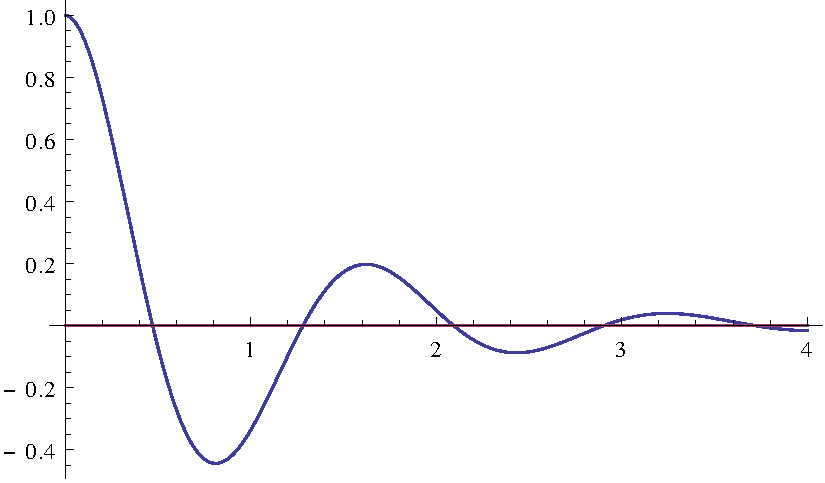
\includegraphics[width=1.1in]{damping2.pdf}\\
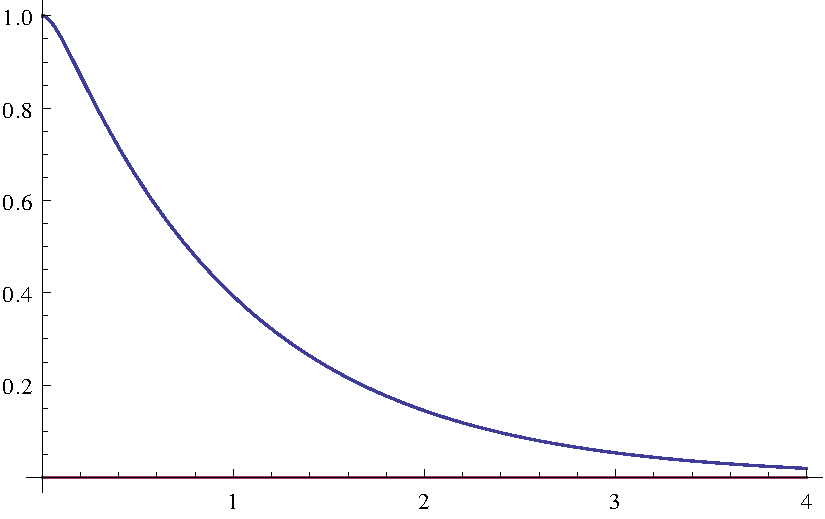
\includegraphics[width=1.1in]{damping17.pdf}\\
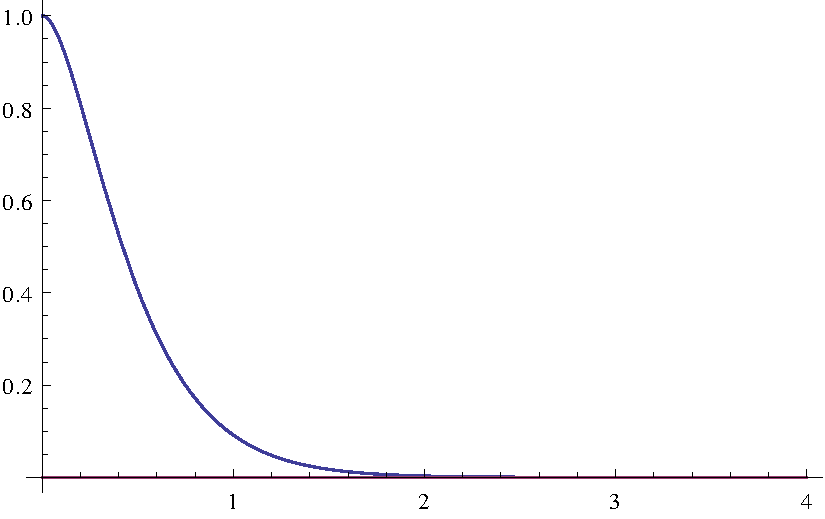
\includegraphics[width=1.1in]{damping8.pdf}\\
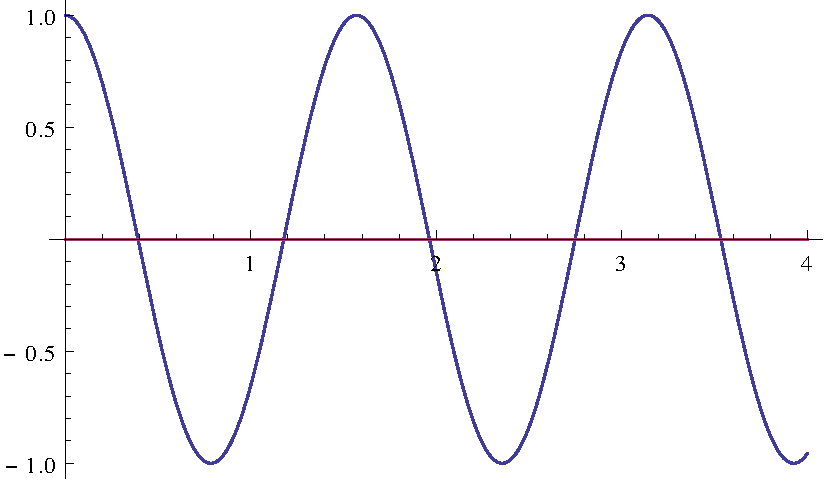
\includegraphics[width=1.1in]{damping0.pdf}
}%
 Recall from the introductory examples that we can model the position of a spring using the ODE $mx''+cx'+kx=0$. 
 We now attach a mass of 1 kg to a spring with $k=16$ kg/s$^2$. We extend the spring 1 cm and then release it.  The spring is inside a dashpot, to add friction to the system, and the dashpot has a coefficient of friction equal to $c$ kg/s. 
\begin{enumerate}
 \item If $c=0$ then a basis for the general solution is $\cos 4t$ and $\sin 4t$.  For each of $c=2,8,17$, state a basis for the general solution (you'll see the irrational number $\sqrt{15}$ when $c=2$).  
 \item The graph of the IVPs for $c=0,2,8,17$ are shown on the right. Match each graph to the correct coefficient of friction. Explain.
 \item As the coefficient of friction increases, describe with a sentence or two what happens to the graph of the solution.
\end{enumerate}

\end{problem}




 We already know that the general solution to the ODE $y''+y=0$ is $y=c_1\cos t+c_2\sin t$. In this problem, we'll discover a crucial identity that connects the trigonometric functions to complex exponentials.

\begin{problem}[Euler's Identity]
 Consider the ODE $y''+y=0$. This models the undamped motion of a spring where $m=1$ and $k=1$.    
\begin{enumerate}
 \item Explain why both $y(t) = c_1\cos t+c_2\sin t$ and also $y(t) = c_3 e^{it}+c_4e^{-it}$ are a general solution to this ODE.
 \item If $y(0)=1$ and $y'(0)=0$, show that $y(t)=\cos t=\dfrac{e^{it}+e^{-it}}{2}$.
 \item If $y(0)=0$ and $y'(0)=1$, show that $y(t)=\sin t=\dfrac{e^{it}-e^{-it}}{2i}$.
 \item The equations $\cos t=\dfrac{e^{it}+e^{-it}}{2}$ and $\sin t=\dfrac{e^{it}-e^{-it}}{2i}$ show us how to write $\cos t$ and $\sin t$ as a linear combination of $e^{it}$ and $e^{-it}$. Use these equations to write $e^{it}$ as a linear combination of $\cos t$ and $\sin t$.  You should obtain values for $A$ and $B$ when you write $e^{it} = A\cos t+B\sin t$. 
\end{enumerate}

\end{problem}










It's time to get back to $AQ=QD$, and show a powerful solution technique. 

\begin{problem}
 Two tanks are connected with hoses and pumps so that 3 gallons/second flows back and forth between the tanks.  The first tank is a 60 gallon tank, with 2 lbs of salt inside.  The second tank is a 90 gallon tank with 23 lbs of salt in it. Please find the amount of salt in each tank at any time $t$. 
\begin{enumerate}
 \item Write a linear system of ODEs in the form 
$$
\begin{pmatrix}
 y_1'\\y_2'
\end{pmatrix}
=
A
\begin{pmatrix}
 y_1\\y_2
\end{pmatrix}.
$$
whose solution will give the amount of salt in each tank at any time $t$.
 \item Compute the eigenvalues and eigenvectors of A, and then write a general solution to this system of ODEs. Your solution should involve arbitrary constants $c_1$ and $c_2$.
 \item Use the initial conditions to solve for $c_1$ and $c_2$.
 \item 
\marginpar{You can check your work with technology.  \href{http://bmw.byuimath.com/dokuwiki/doku.php?id=systems_of_odes_grapher}{Follow this link.} }%
Construct a graph that contains the the vector field representing the coefficient matrix and the parametric plot $\vec y(t) = (y_1(t),y_2(t))$ of your solution.
\end{enumerate}

\end{problem}


\begin{problem}
 Consider the linear system of ODEs given by $y_1'=2y_1+y_2$ and $y_2'=3y_1+4y_2$. Let $\vec y = (y_1,y_2)$. We can write this ODE in the form $\vec y' = A\vec y$, where $\vec y = (y_1,y_2)$.  
 \begin{enumerate}
  \item Find the eigenvalues of $A$.  Then give a basis for each eigenspace.
  \item We know that we can write a general solution to this system of ODEs as 
$$
\vec y=
c_1\vec x_1 e^{\lambda_1 t }+c_2\vec x_2 e^{\lambda_2 t}.
$$
Find a 2 by 2 matrix $Q$ so that we can write this solution in the form 
%\marginpar{Hint: Expand the product of the matrices. You'll see what $Q$ must be.}
$$
\vec y=
Q\begin{bmatrix}
 e^{\lambda_1 t} & 0\\
 0 & e^{\lambda_2 t}
\end{bmatrix}
\begin{bmatrix}
c_1\\c_2 
\end{bmatrix}
=QD\vec c,
$$
where we have $D=
\begin{bmatrix}
 e^{\lambda_1 t} & 0\\
 0 & e^{\lambda_2 t}
\end{bmatrix}$ 
and  
$\vec c =
\begin{bmatrix}
c_1\\c_2 
\end{bmatrix}
$.
\item We now have $\vec y = QD\vec c$. When we let $t=0$, explain why $D$ equals the identity matrix. This means that $\vec y(0) = Q\vec c$.  Solving for $\vec c$ gives us $\vec c= Q^{-1}\vec y(0)$.  Compute the inverse of $Q$.
 \item \marginpar{You can check your work with technology.  \href{http://bmw.byuimath.com/dokuwiki/doku.php?id=systems_of_odes_grapher}{Follow this link.} }%
Since we know $\vec y = QD\vec c$ and $\vec c= Q^{-1}\vec y(0)$, this means 
$$\vec y = QDQ^{-1}\vec y(0).$$
You have found $Q$, $D$, and $Q^{-1}$. If we let $y_1(0)=a$ and $y_2(0)=b$ which means $\vec y(0)=(a,b)$, then multiply out the matrix product $QDQ^{-1}\vec y(0)$ and state the solution to this IVP.
\end{enumerate}

\end{problem}

In the problem above, we solved the linear system of ODEs in the form $\frac{d\vec y}{dt} = A\vec y$  with initial conditions $\vec y(0)$ by just writing
$$\vec y = QDQ^{-1}\vec y(0).$$
The columns of $Q$ are the eigenvectors. The nonzero entries of the diagonal matrix $D$ contain $e^{\lambda t}$ where $\lambda$ is an eigenvalue.  Does this pattern work in other places?

\begin{problem}
 \marginpar{You can check your work with technology.  \href{http://bmw.byuimath.com/dokuwiki/doku.php?id=systems_of_odes_grapher}{Follow this link.} }%
 Solve the system of ODEs $\frac{d\vec y}{dt} = A\vec y$ where 
$A
=\begin{bmatrix}
  6&2\\2&3
 \end{bmatrix}
$. Do so by stating $Q$, $D$, and $Q^{-1}$, and then perform the matrix product $QDQ^{-1}$. Finally, if we assume $\vec y(0) = (a,b)$, then give the solution to this system of IVPs by stating what $y_1(t)$ equals, and what $y_2(t)$ equals (hint, multiply out $QDQ^{-1}\vec y(0)$  ).  Please use technology to perform as much of the computations as you want. Just be prepared to tell us how you got each part.
\end{problem}

Does the pattern above continue to work if we increase the size of the matrix?
\begin{problem}
 \marginpar{You can check your work with technology.  \href{http://bmw.byuimath.com/dokuwiki/doku.php?id=systems_of_odes_grapher}{Follow this link.} }%
 Solve the system of ODEs $\vec y '=A\vec y$ where 
$A
=\begin{bmatrix}
  2&1&1\\1&2&0\\0&0&4
 \end{bmatrix}
$. Do so by stating $Q$, $D$, and $Q^{-1}$, and then perform the matrix product $QDQ^{-1}$. Finally, if we assume $\vec y(0) = (a,b,c)$, then give the solution to this system of IVPs by stating what $y_1(t)$ equals, what $y_2(t)$ equals, and what $y_3(t)$ equals. Please use technology to perform as much of the computations as you want. Just be prepared to tell us how you got each part.
\end{problem}

Does the pattern even work if the eigenvalues are complex?
\begin{problem}
 Solve the system of ODEs $\vec y '=A\vec y$ where 
$A
=\begin{bmatrix}
  0&1\\-1&0
 \end{bmatrix}
$. 
\begin{enumerate}
 \item Find the eigenvalues by hand.  Then for each eigenvalue, compute an eigenvector by hand. State $Q$ and $D$ from this information.  You are welcome to use $e^{it}$ in your work as needed. 
 \item Compute $Q^{-1}$ by hand.  Then compute the product $QDQ^{-1}$ by hand.
 \item 
\marginpar{Why does $\cos(-t)=\cos t$ and $\sin(-t)=-\sin t$?}%
Use Euler's formula $e^{it} = \cos t +i\sin t$ to simplify the product $QDQ^{-1}$. You should be able to simplify the product to remove all complex terms. Note that $e^{-it}=e^{i(-t)} = \cos(-t) +i\sin(-t)=\cos(t)-i\sin(t)$.
 \item 
\marginpar{You can check your work with technology.  \href{http://bmw.byuimath.com/dokuwiki/doku.php?id=systems_of_odes_grapher}{Follow this link.} }%
If $y_1(0)=5$ and $y_2(0)=7$, then what are $y_1(t)$ and $y_2(t)$. Then use software to check your answer. You should see that the solution in the $y_1y_2$ plane, along with the appropriate vector field, gives circular motion.
\end{enumerate}

\end{problem}

\begin{problem}
Suppose that $\frac{d\vec y}{dt} = A\vec y$ is a linear system of ODEs.  Also suppose that $\vec y=\vec x e^{ct}$ is a nonzero solution to this system. Explain, using the definition of eigenvalues and eigenvectors, why we must have that $c$ is an eigenvalue, and $\vec x$ is an eigenvector corresponding to $c$. [Hint:  Look up the definition of eigenvalues and eigenvectors.  If you compute $\frac{d\vec y}{dt}$ and then place both $\vec y$ and $\frac{d\vec y}{dt}$ into the system $\frac{d\vec y}{dt}= A\vec y$, you should see the definition appear.] 
\end{problem}













In the previous sections, we focused mainly on second order ODEs.  We started by using Laplace transforms to find the exact solutions.  The accompanying partial fraction decomposition was sometimes rather ugly, so we opted for guessing the form of the solution, and then taking derivatives to determine the unknown constants. 

\begin{problem}
 Consider the ODE $y'''+3y''+3y'+y=0$ (where $y$ is a function of $x$, not $t$).  Compute the Laplace transform of both sides, and solve for $Y$.  The denominator factors as $(s+1)^3$. Explain why a general solution is $y = c_1 e^{-x}+c_2 x e^{-x}+c_3 x^2e^{-x}.$ 

 For the ODE $y''''+4y'''+6y''+4y'+y=0$, whose characteristic equation is $(s+1)^4=0$, make a guess as to the solution. Then use a computer and dsolve to check that your answer is correct. (Wolfram Alpha can solve this.)

 If you encounter a repeated root, what does that contribute to the solution? Explain this in a way that you and others can remember it. Write a few sentences, and give an example. 
\end{problem}




\begin{problem}
 In each problem below, you are given the characteristic equation of an ODE. State the general solution of the ODE.
\begin{enumerate}
 \item $(s+3)(s+2)(s+1)=0$
 \item $(s+3)(s+3)(s+1)=0$
 \item $(s+3)^3(s^2+9)=0$
 \item $(s+3)^2(s^2+9)^2=0$
 \item $(s+3)^2(s^2-9)^2=0$ (Note the sign change.)
\end{enumerate}
\end{problem}





When we find a basis of solutions for an ODE, we need to know that the functions are linearly independent.  If they are not linearly independent, then they are not a basis. Is there a simple way to determine if solutions are linearly independent?  For example, how do we know that for a 3rd order ODE whose characteristic equation is $(s+3)(s+2)(s+1)=0$ that the functions $e^{-t}$, $e^{-2t}$, and $e^{-3t}$ are linearly independent?  Can we use matrices and determinants to tackle this?  The answer is yes, and its proof is beyond the scope of our class.  The problem is that we need a 3 by 3 matrix matrix from the three functions.
\begin{definition}[Wronskian]
 The Wronskian of a collection of $n$ functions is the determinant of an $n$ by $n$ matrix that we form by placing the functions in the first row and then each other row is the derivative of the row above.  This gives us the Wronskian as
$$W(y_1,y_2) = 
\begin{vmatrix}
 y_1&y_2\\
 y_1'&y_2'
\end{vmatrix}
,\quad
W(y_1,y_2,y_3) = 
\begin{vmatrix}
 y_1&y_2&y_3\\
 y_1'&y_2'&y_3'\\
 y_1''&y_2''&y_3''
\end{vmatrix},
\quad \text{etc.}$$
\end{definition}

\begin{problem}
 For each collection of functions below, compute the Wronskian. Then decide if the functions are linearly independent or linearly dependent.
\begin{enumerate}
 \item $e^{3t}$ and $4e^{3t}$
 \item $\cos t$ and $\sin t$
 \item $e^t$, $e^{2t}$, and $e^{3t}$
 \item $\cosh t$, $\sinh t$, and $e^{t}$ (Simplify this one fully.)
 \item What does the Wronskian equal if the functions are linearly dependent?
\end{enumerate}
You should have found that two were dependent, and two were independent. 
\end{problem}




\section*{Wrap up}
\addcontentsline{toc}{section}{Wrap Up}

This concludes the chapter.  Look at the objectives at the beginning of the chapter. Can you now do all the things you were promised? 


\begin{problem}[Lesson Plan Creation] \marginpar{This counts as 4 prep problems. My hope is that you spend at least an hour creating your one-page lesson plan.}
Your assignment: organize what you've learned into a small collection of examples that illustrates the key concepts. I'll call this your one-page lesson plan. You may use both sides. The objectives at the beginning of the chapter give you a list of the key concepts. Once you finish your lesson plan, scan it into a PDF document (use any scanner on campus), and then upload the document to I-Learn.
\end{problem}



